\section{Methods}

TODO

\subsection{TODO}


As described in \citep{TODOcitedishtinygp}.

Fledgling interconnects with two prongs.
Each prong performs a random walk over kin groups, accumulating positive or negative based on tag-matching with tags expressed by underfoot cells.
Prongs that get too far behind jump to the location of the better-scoring prong.
Once a score threshold has been reached, the best-scoring prong develops into a full-fledged connection.
At this point, the originating cell can begin sending messages and/or resource over the connection to the TARGEt cell.
The TARGet cell can also send messages back to the originating cell.
These behaviors are triggered by execution of special instructions.
(A full listing of instructions is available in supplementary todo ref.)

Each cell contains four SignalGP instances that manage behavior with respect to each direction.
For these experiments, we added a fifth SignalGP instance to manage behavior with respect to interconnect.
Directional SignalGP instances may also broadcast messages over the interconnects.
Broadcast messages received over the interconnect are de-duplicated before being distributed instances within a receiving cell.

You can see this developmental process in action in an evolved strain at \url{https://mmore500.com/hopto/ap}.

\begin{figure}[t]
\begin{center}
%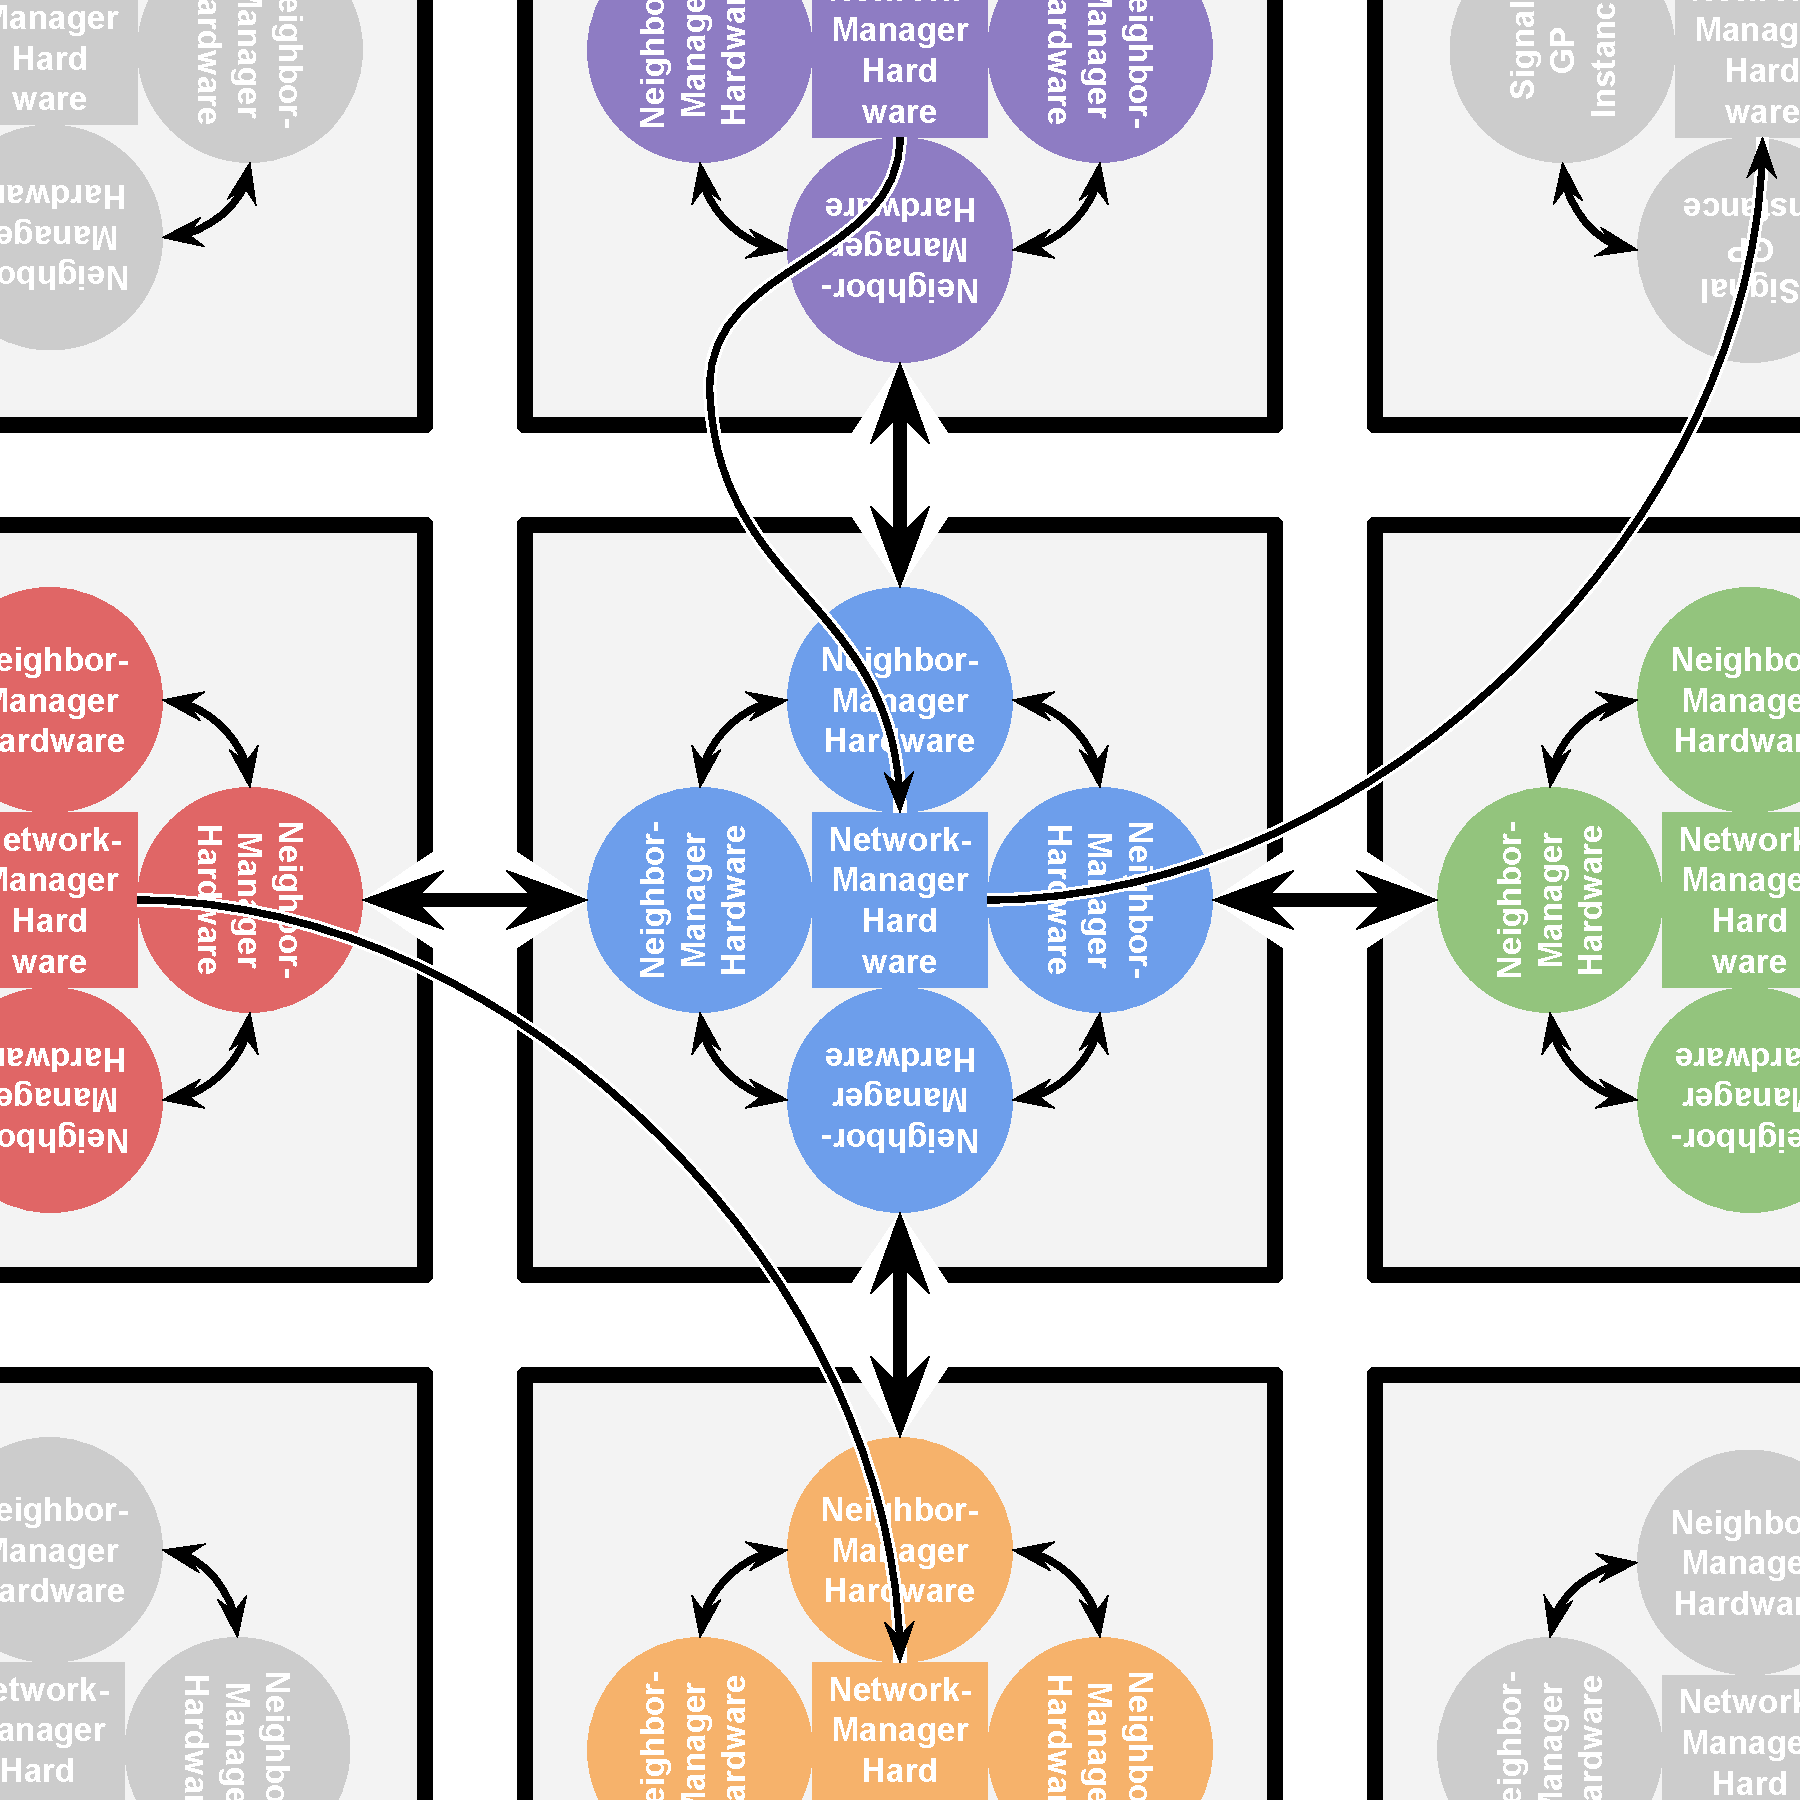
\includegraphics[width=0.7\linewidth]{img/spiker-pointer-hardware.pdf}
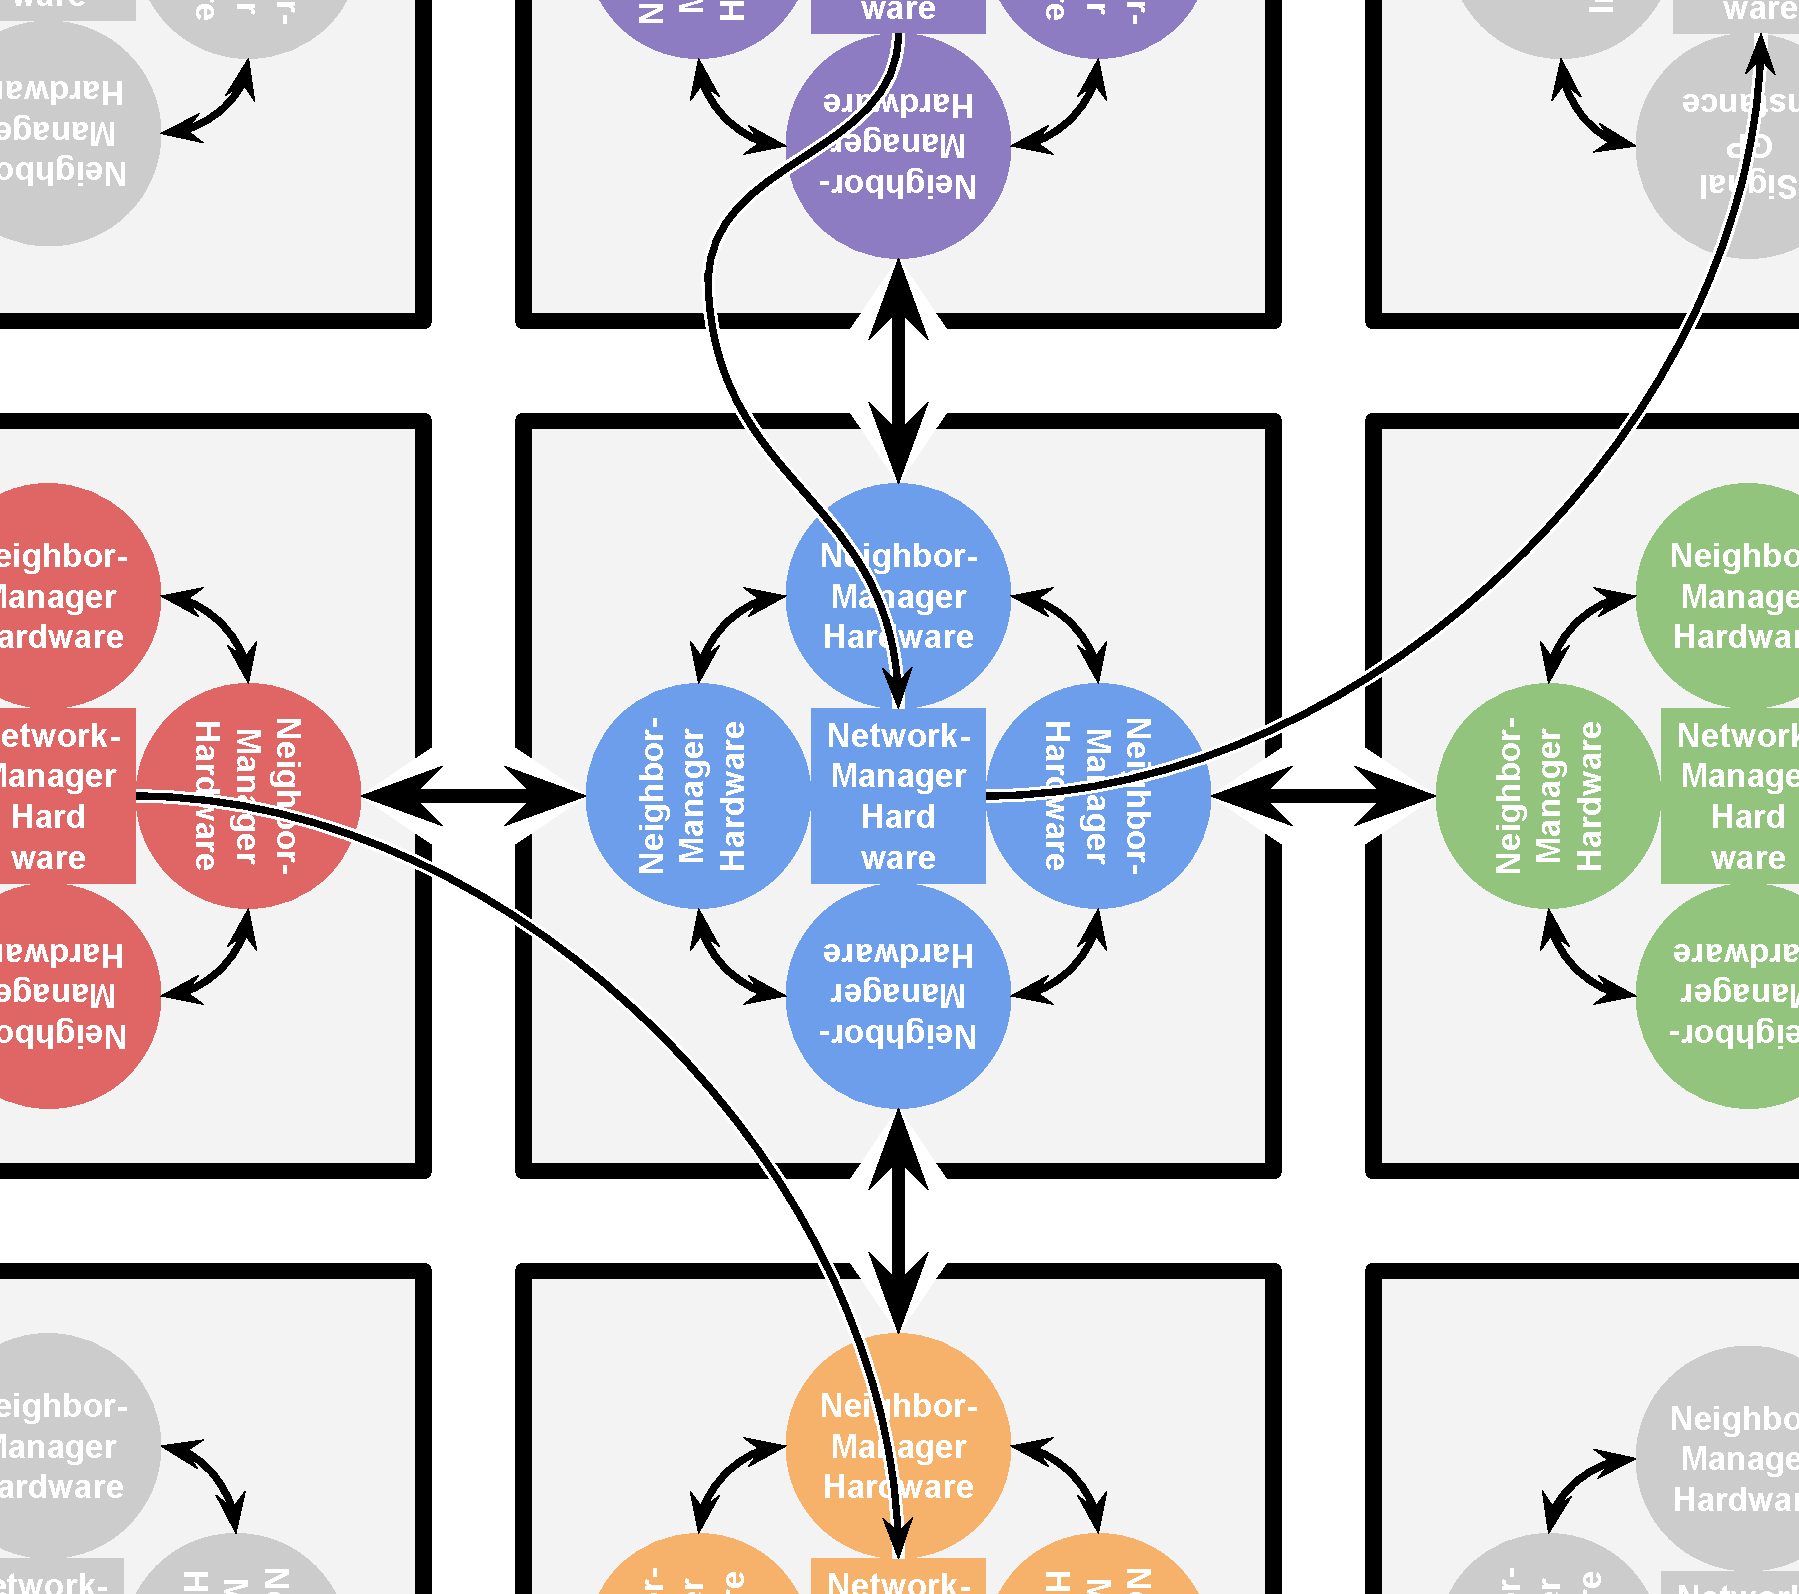
\includegraphics[width=0.8\linewidth]{img/spiker-pointer-hardware2.pdf}
\caption{
Arrangement of SignalGP hardware within DISHTINY cells (gray squares).
Neighbor-managing hardware (circles) receive stimuli and control cell behavior with respect to a particular cell neighbor.
Network-managing hardware (interior squares) receive stimuli and controll cell behavior with respect to more distant neighbors a cell has established interconnects with.
}
\label{fig:spiker_pointer_hardware}
\end{center}
\end{figure}


\begin{figure*}[!htbp]
\begin{center}
\begin{subfigure}[b]{0.33\linewidth}
  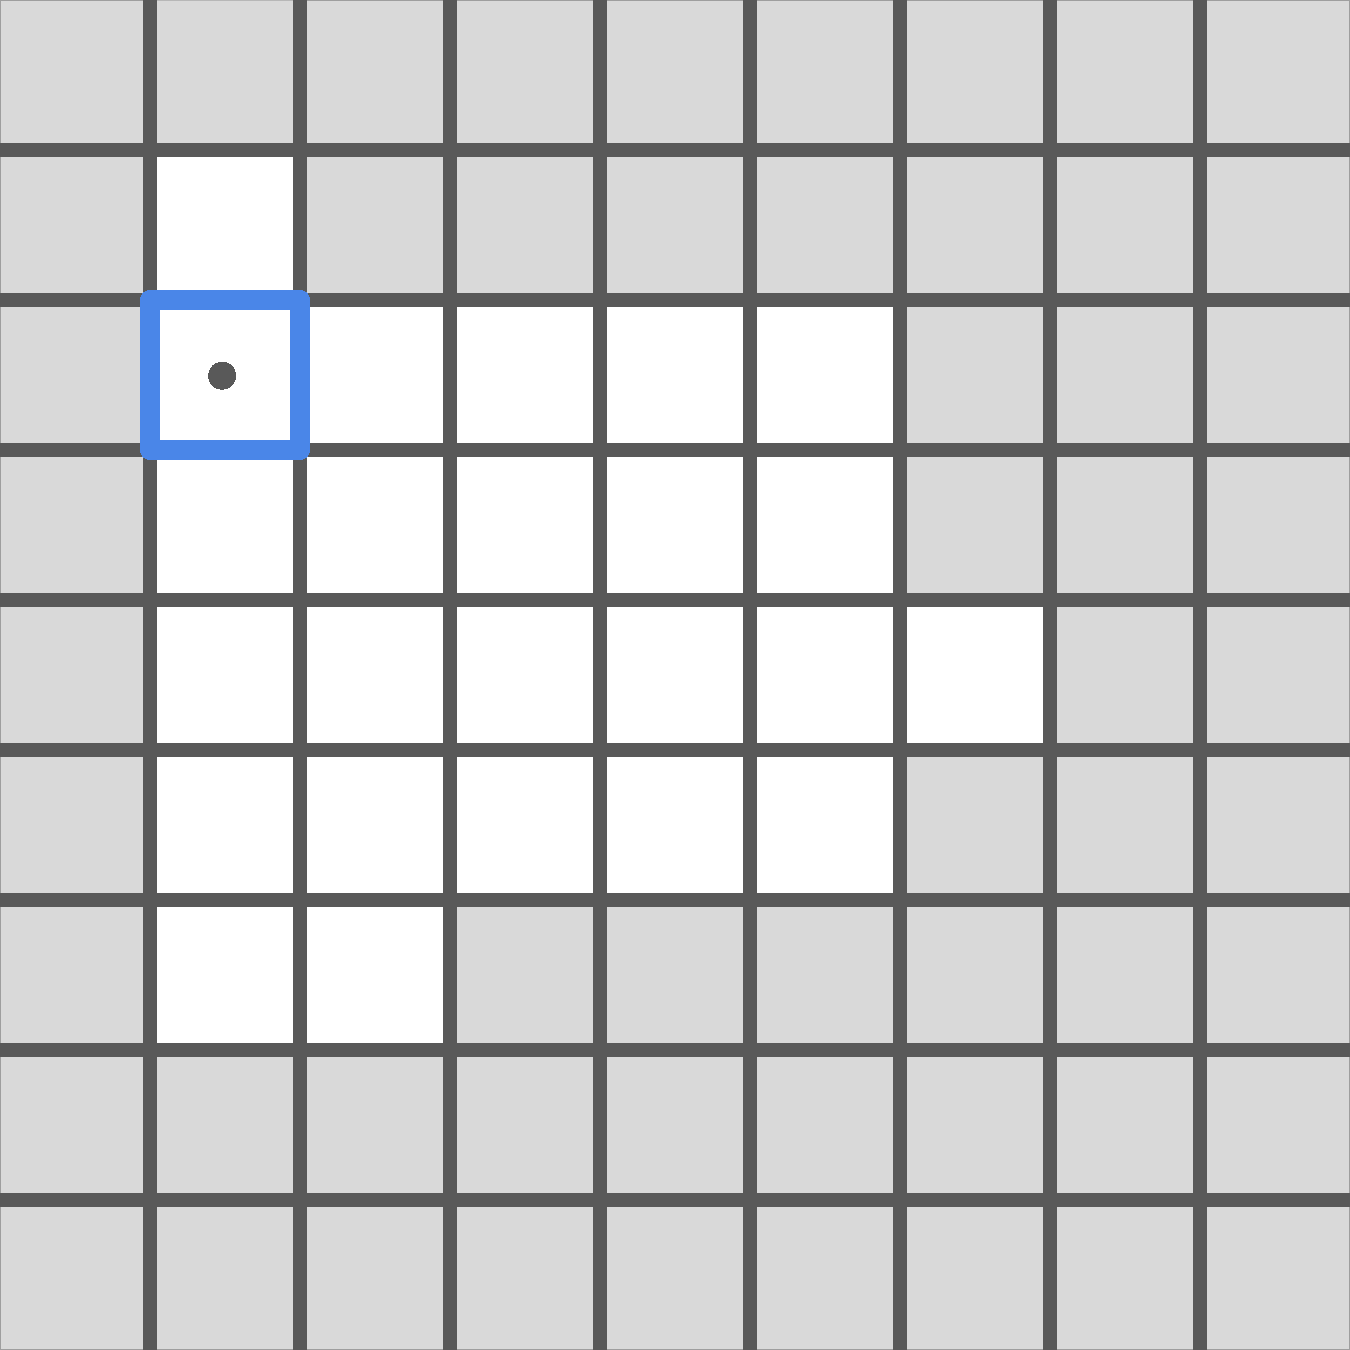
\includegraphics[width=\linewidth,trim={0 100 100 0},clip]{spiker-diagram/spiker-generate}
  \caption{TODO}
  \label{fig:TODO}
\end{subfigure}
\begin{subfigure}[b]{0.33\linewidth}
  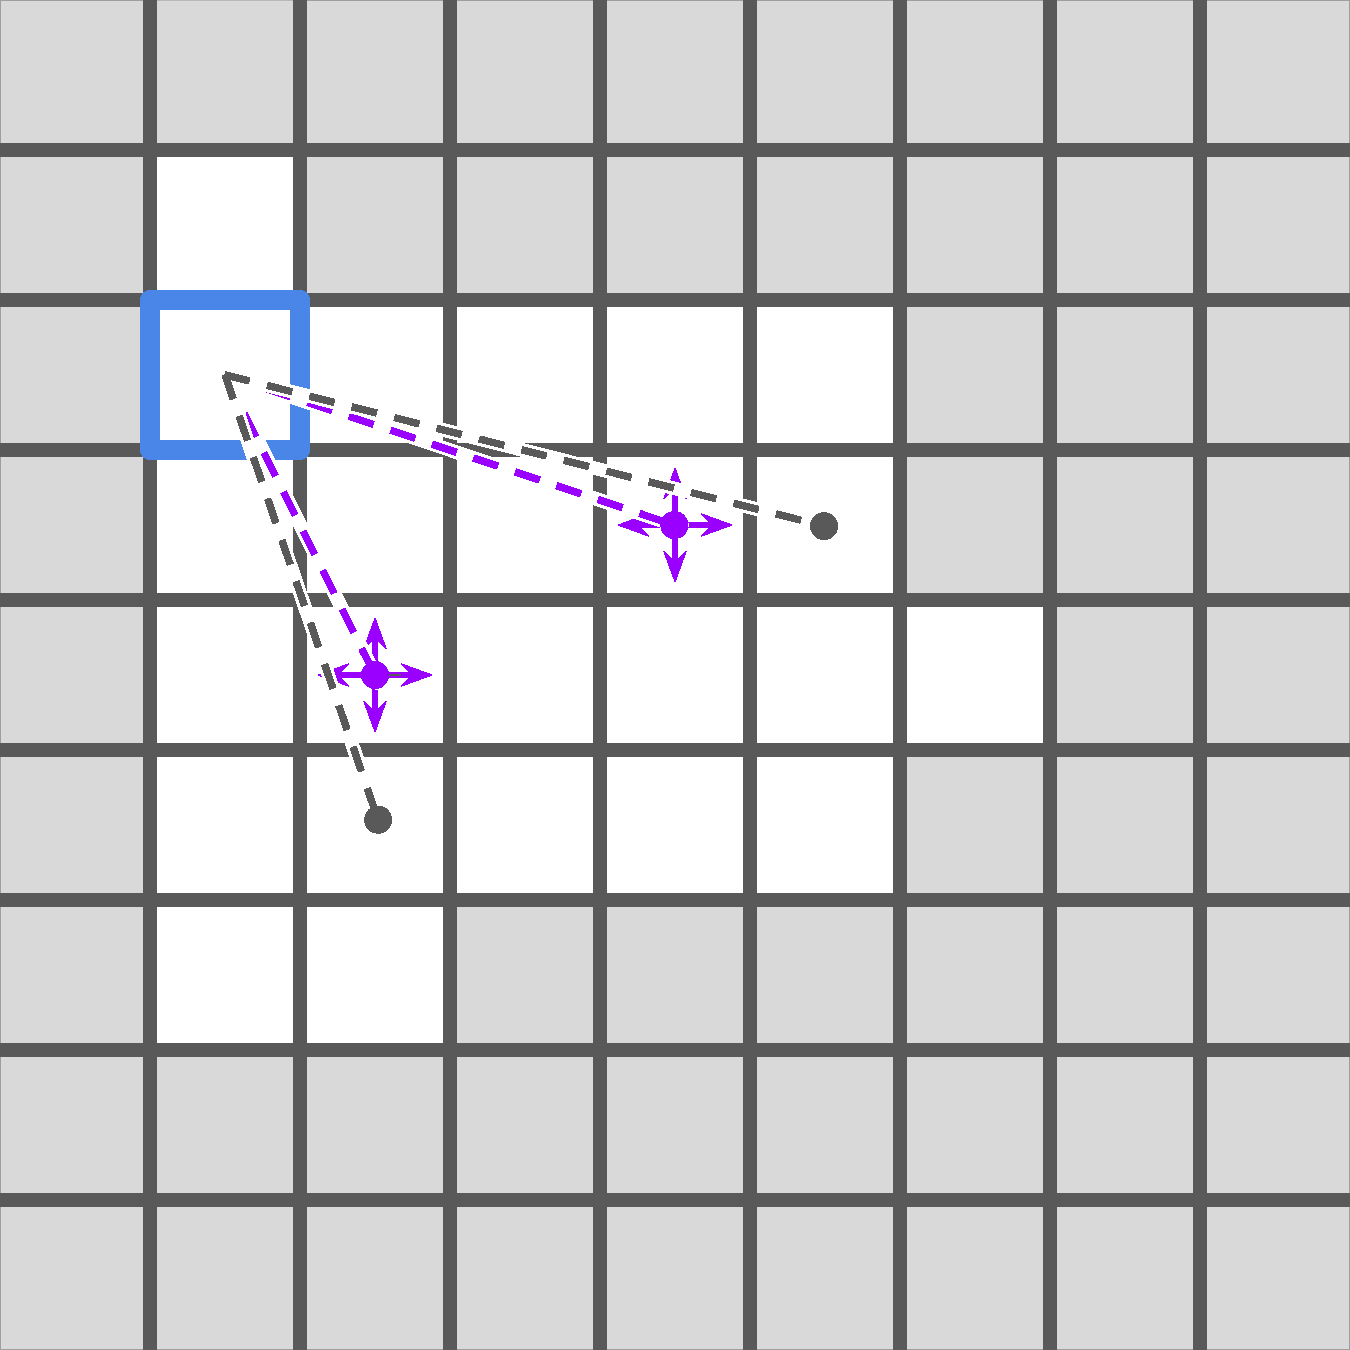
\includegraphics[width=\linewidth,trim={0 100 100 0},clip]{spiker-diagram/spiker-walk}
  \caption{TODO}
  \label{fig:TODO}
\end{subfigure}
\begin{subfigure}[b]{0.33\linewidth}
  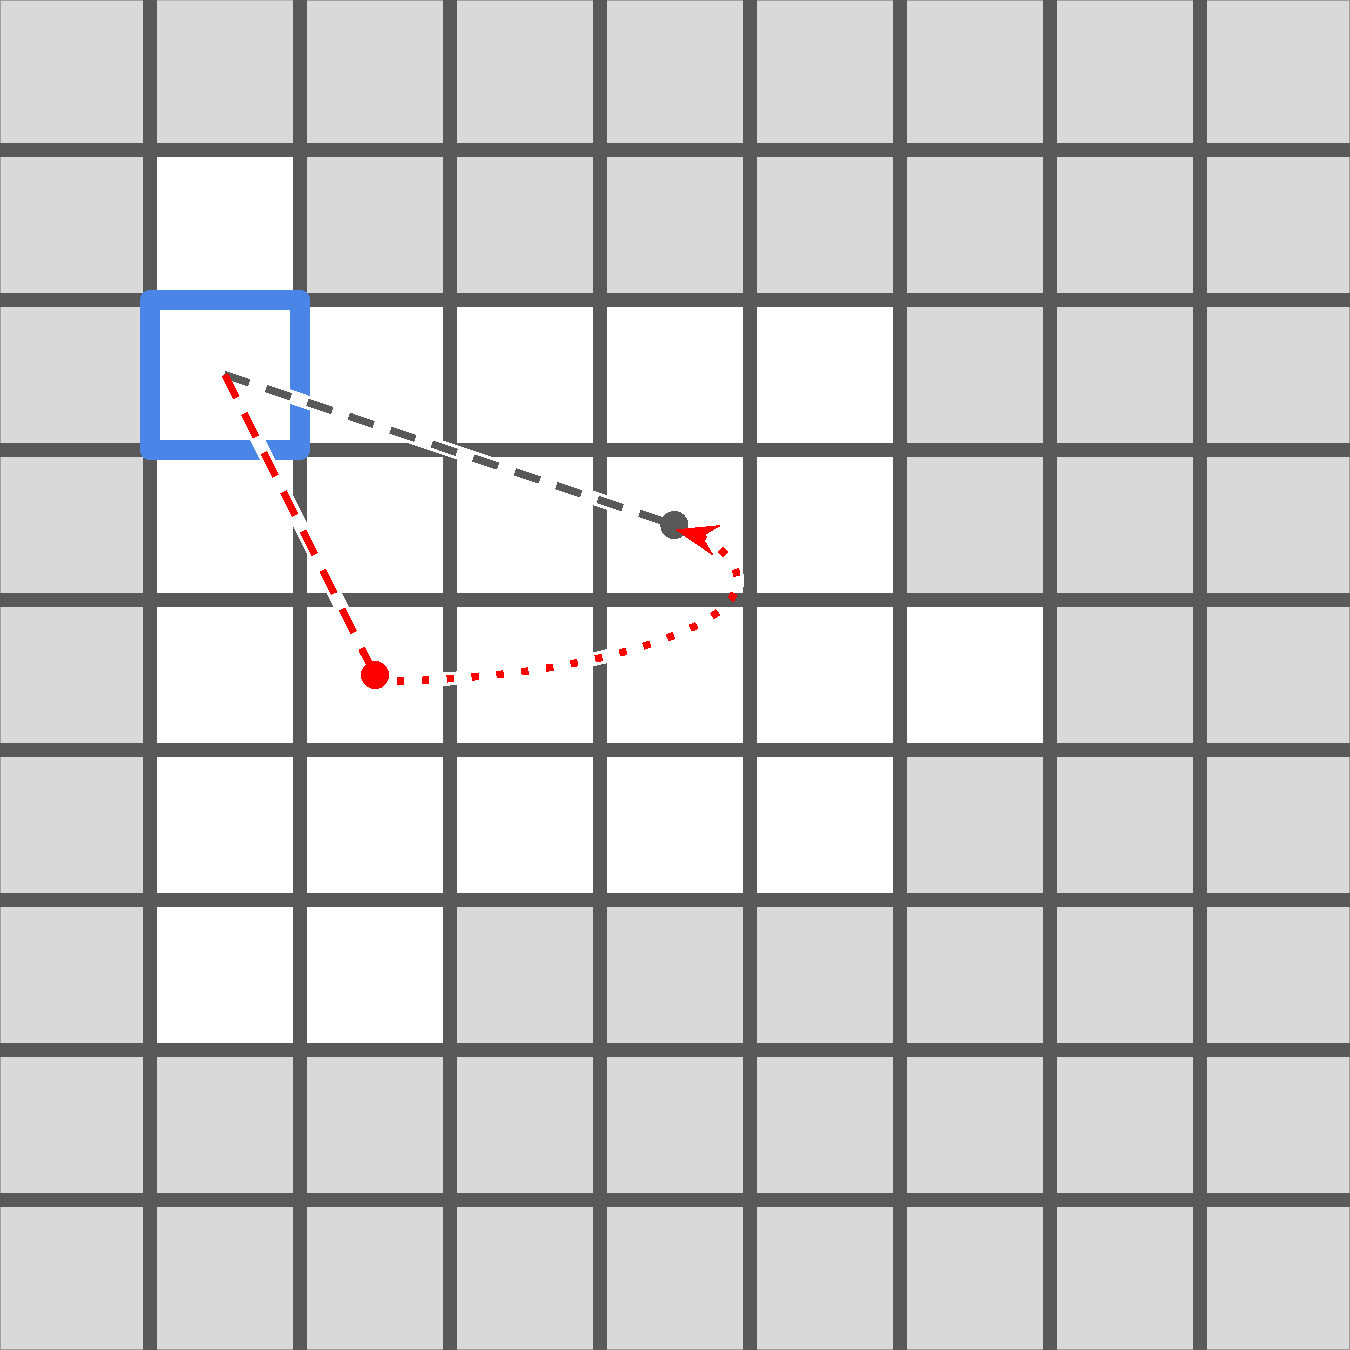
\includegraphics[width=\linewidth,trim={0 100 100 0},clip]{spiker-diagram/spiker-swap}
  \caption{TODO}
  \label{fig:TODO}
\end{subfigure}
\begin{subfigure}[b]{0.33\linewidth}
  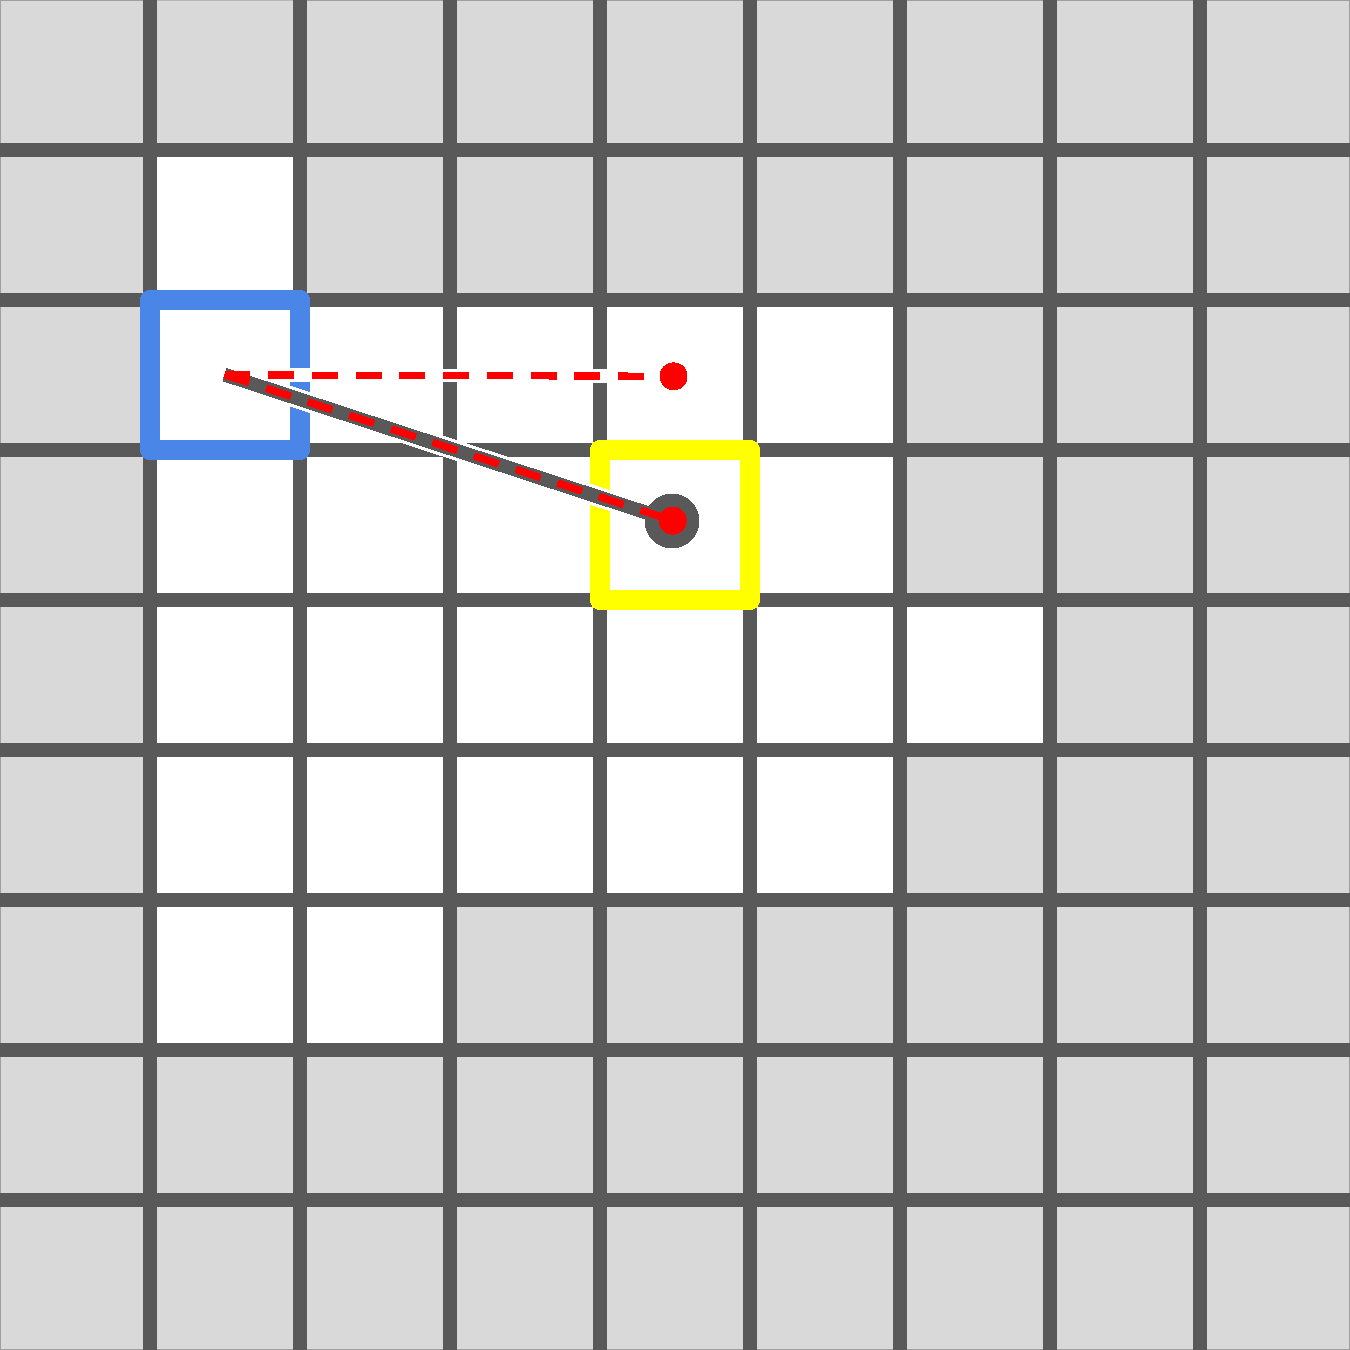
\includegraphics[width=\linewidth,trim={0 100 100 0},clip]{spiker-diagram/spiker-connect}
  \caption{TODO}
  \label{fig:TODO}
\end{subfigure}
\begin{subfigure}[b]{0.33\linewidth}
  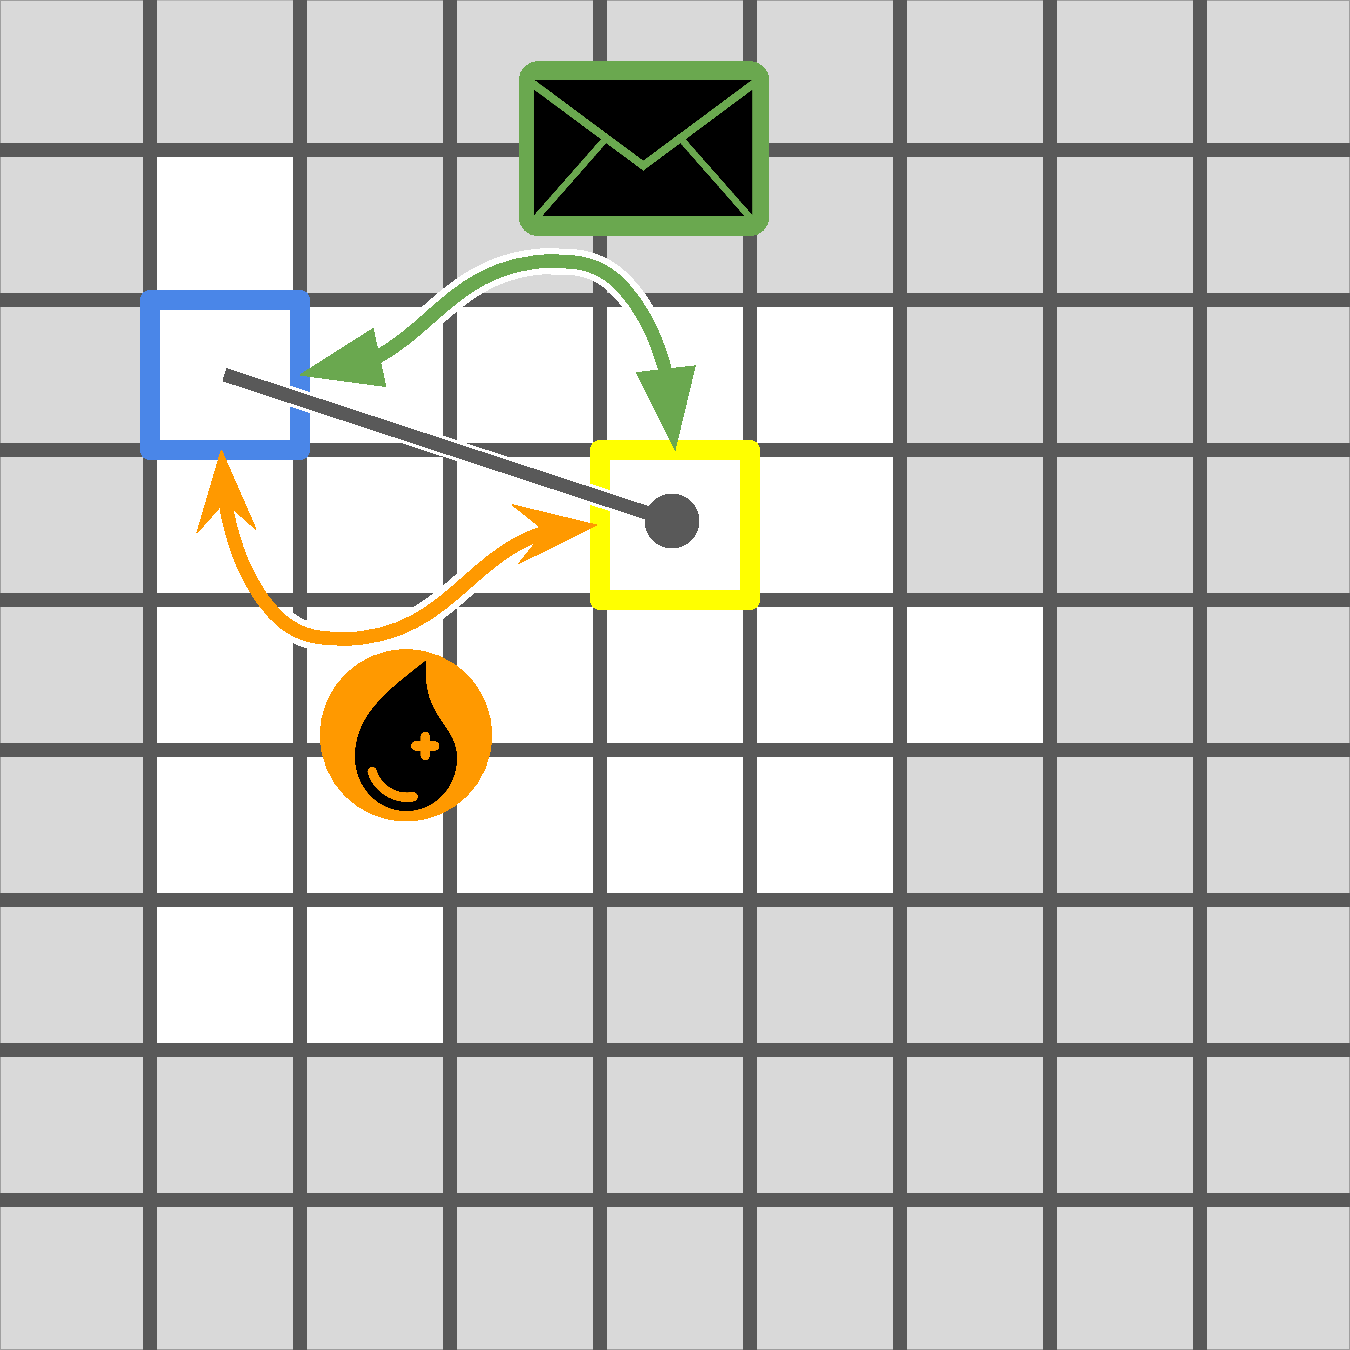
\includegraphics[width=\linewidth,trim={0 100 100 0},clip]{spiker-diagram/spiker-transmit}
  \caption{TODO}
  \label{fig:TODO}
\end{subfigure}
\begin{subfigure}[b]{0.33\linewidth}
  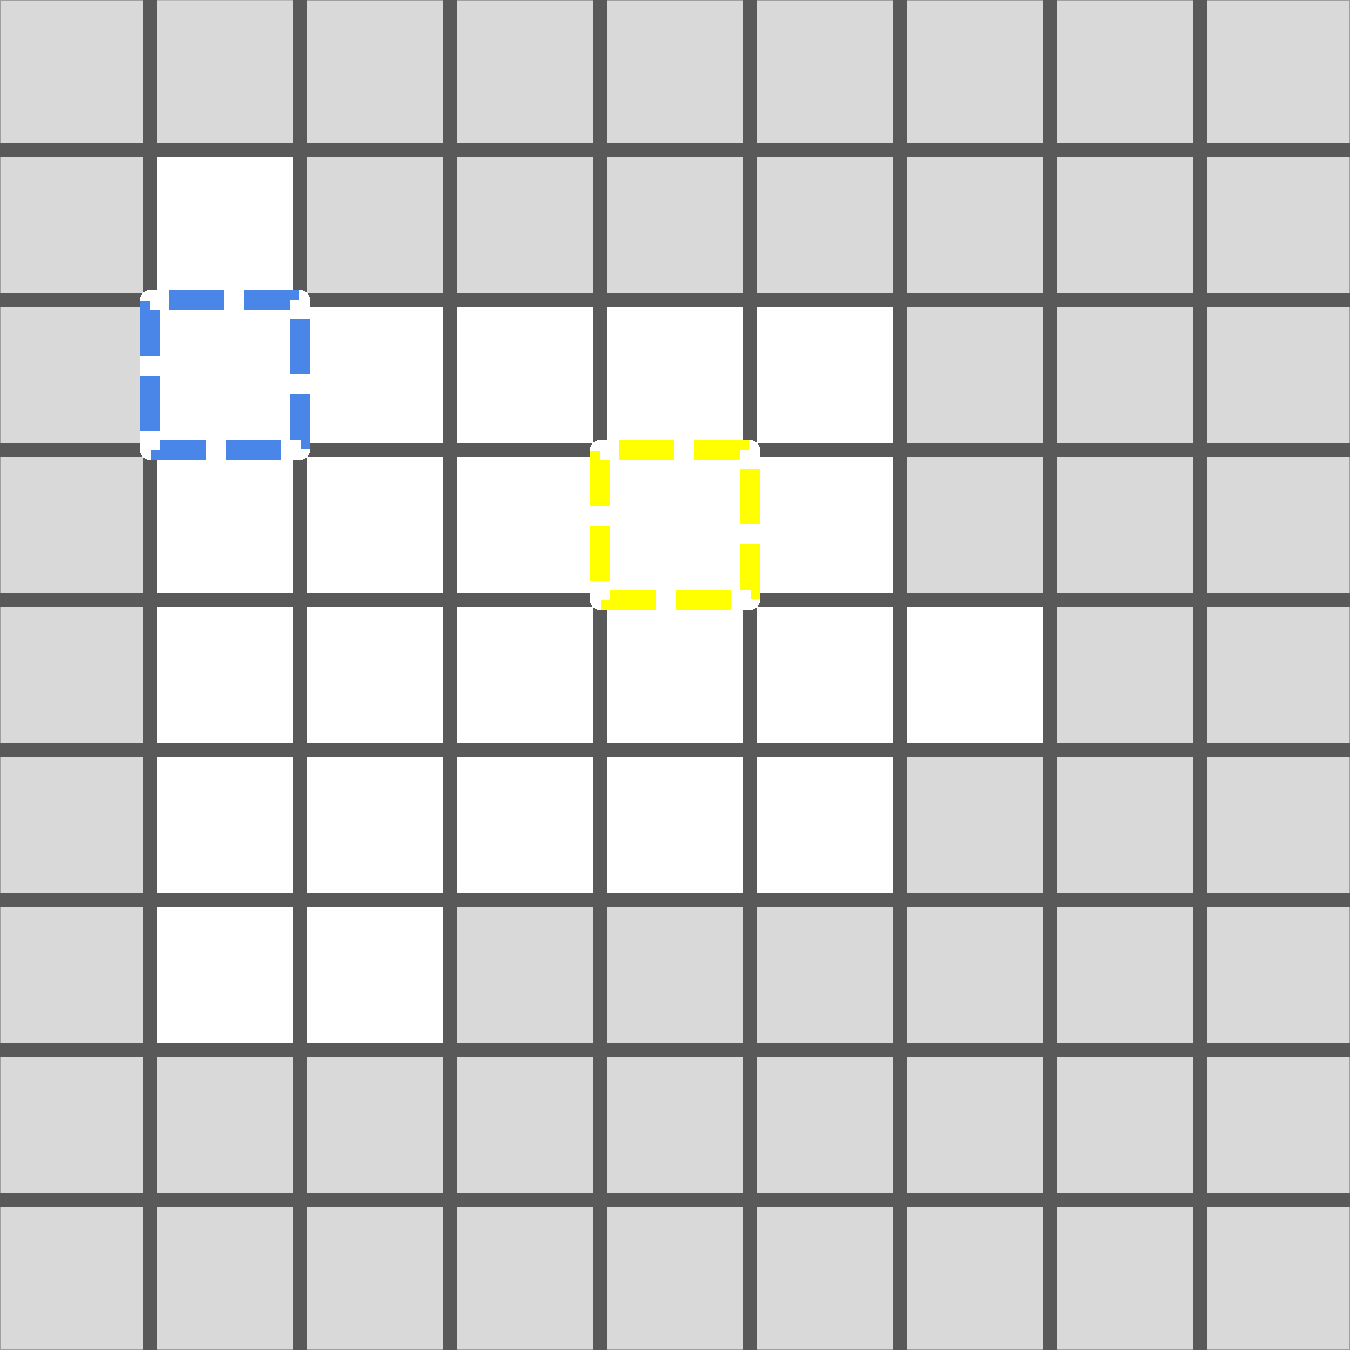
\includegraphics[width=\linewidth,trim={0 100 100 0},clip]{spiker-diagram/spiker-remove}
  \caption{TODO}
  \label{fig:TODO}
\end{subfigure}
\caption{
TODO
}
\label{fig:spiker_diagram}
\end{center}
\end{figure*}


\subsection{Evolutionary Screens}

We running 64 replicate batches in 4-hour steps.
Each batch consisted of four isolated subpopulations, which were completely intermixed in between four-hour steps.

We screened across four-hour checkpoints of replicate batches to see if messages or resource were being sent over interconnects.
We sampled from these populations, performing screens for knockouts of interconnect messaging or resource sharing.
We found several evolved genotypes that used interconnects adaptively.
We then further screened to ensure that the intra-cellular nature of the interconnects were vital by testing to see whether connecting interconnects to the originating cells themselves after the developmental process affected fitness.

We continued this process until we found a strain where interconnects were used for resource sharing and a strain where interconnects were used for cell-cell messaging.

We did not find a strain where resource sharing was used outside of the context of interconnect resource sharing in the main set of set or runs.
So we performed a secondary set of runs with several adjustments and different seeds, including:
\begin{enumerate}
  \item increasing the default outgoing connection cap and
  \item making cells default-accept instead of default-reject intracellular messages from same-channel cells.
\end{enumerate}

We repeated the screening process on the secondary process, finding a strain where interconnects were used for adaptive cell-cell messaging outside the context of resource sharing over the interconnect.

\subsection{Implementation}

We implemented our experimental system using the Empirical library for scientific software development in C++, available at \url{https://github.com/devosoft/Empirical} \citep{TODOcite}.
We used OpenMP to parallelize our main evolutionary replicates, distributing work over two threads.
The code used to perform and analyze our experiments, our figures, data from our experiments, and a live in-browser demo of our system is available via the Open Science Framework at \url{https://osf.io/TODO/}.
